\section{State-of-the-art Text-To-SQL Methods}

\begin{figure}[htb]
    \centering
    \includegraphics[width=0.99\textwidth]{pics/Timeline.png}
    \caption{Timeline of the deep learning process for Text-to-SQL.}
    \label{fig:timeline}
\end{figure}

This section will discuss existing cross-domain state-of-the-art (SOTA), text-to-SQL models, beginning with a broad overview and moving on to individual modules. This will provide a clear picture of the progress made in text-to-SQL research. Experiments have shown that pre-trained embeddings improve models because they construct better schema linking and a more accurate SQL structure.

An efficient text-to-SQL solution requires state-of-the-art natural language processing techniques.
As a result of the neural network's ability to handle only numerical inputs and not raw text, word embedding has been used to represent numerical words.
Aside from that, in the past few years, language models have become increasingly popular as a solution for increasing performance in natural language processing tasks.
Assuming that words have numerical representations that differ from those of other words, word embeddings aim to map each word to a multidimensional vector, incorporating valuable information about the word. In addition to the brute-force creation of one-hot embeddings, researchers have developed highly efficient methods for creating representations that convey a word's meaning and relationships with other words. In most, if not all, Text-to-SQL systems, word embedding techniques such as Word2Vec\cite{DBLP:journals/corr/Rong14}, and WordPiece embeddings\cite{DBLP:journals/corr/WuSCLNMKCGMKSJL16} are used.

Recently Language models have been shown to excel at NL tasks as a new type of pre-trained neural network. It is important to note that language models are not a replacement for word embeddings since they are neural networks and need a way to transform words into vectors.
Depending on the specific problem they want to solve, researchers can adapt the pre-trained model's inputs and outputs and train it for an additional number of epochs on their dataset. Thus, we can achieve state-of-the-art performance without complex architectures \cite{DBLP:journals/corr/abs-1810-04805}. Recent neural network architectures, like the Transformer\cite{DBLP:journals/corr/VaswaniSPUJGKP17}, have been used to achieve such performance by these models, which excel at handling NL and sequences of NL that are characterized by connections between words. Several language models have been used to handle the text-to-SQL task, including BERT \cite{DBLP:journals/corr/abs-1810-04805}. BERT is a pre-trained language model that has been shown to achieve state-of-the-art performance in a variety of NLP tasks. BERT is a Transformer-based model that uses a bidirectional encoder to learn the representation of a word based on the context in which it appears. BERT has been used in several text-to-SQL models, such as BRIDGE \cite{lin_bridging_2020} and RAT-SQL \cite{wang_rat-sql_2021}.

\subsection{Sequence-to-SQL}

\subsubsection{Seq2Seq}

In natural language processing, Sequence-to-Sequence (Seq2Seq)\cite{DBLP:journals/corr/SutskeverVL14} models are a type of neural network architecture used for tasks such as machine translation, text summarization, and text-to-speech conversion. These are the two main components of the model. Encoders and decoders make up the core of the Seq2Seq model. The encoder receives a stream of data as input, such as a sentence written in one language, and transforms it into a representation with a fixed length, which is also referred to as the hidden state. This concealed state is then sent to the decoder, which is responsible for generating the output sequence, which may include the sentence being translated into a different language.

There are a variety of methods that can be used to train Seq2Seq models, such as supervised learning, in which the model is trained on a dataset of input-output pairs, and unsupervised learning, in which the model is trained to reconstruct the input sequence. Both of these methods are examples of how the model can be trained. Attention mechanisms, such as the attention mechanism used in the Transformer model, can also be incorporated into Seq2Seq models to improve their performance. This is accomplished by allowing the decoder to focus selectively on certain parts of the input sequence. Attention mechanisms can also be used in the Transformer model.

Natural language processing applications make extensive use of Seq2Seq models because of their versatility in managing sequences of varying lengths, both in terms of input and output and also in terms of the data they process sequentially. However, one of the most significant difficulties associated with Seq2Seq models is the possibility of producing outputs that are irrelevant or need to be clarified. This issue is referred to as the "exposure bias" problem. Researchers have come up with several potential solutions to this issue, including using beam search while the model is being trained or training the model with scheduled sampling.

% image of seq2seq.png
\begin{figure}[ht]
    \centering
    \includegraphics[width=0.5\textwidth]{pics/seq2seq.png}
    \caption{Example of Seq2Seq model in translating a sentence from English to French.}
    \label{fig:seq2seq}
\end{figure}

\subsubsection{Seq2SQL}

An output of a sequence-to-sequence approach is a sequence of SQL tokens and schema elements, with that sequence being used to predict SQL queries or at least a significant portion of them. An NLQ sequence is transformed into a SQL sequence by these programs. There is no doubt that this approach is the simplest, but it is also the most error-prone. Seq2SQL\cite{zhong_seq2sql_2017}, one of the first deep-learning systems, used this approach, but later, systems avoided it. sequence-to-sequence architectures have the major disadvantage of not taking the strict grammar rules of SQL into account when generating queries.

As part of this model, its authors released the WikiSQL dataset, which ushered in a new era of text-to-SQL deep learning research. GloVe embeddings represent the inputs in the network architecture, which combines LSTM and linear layers. With a seq-to-seq network, the system predicts the aggregation function and the column for the SELECT clause. Its major drawback is that it generates parts of the query that can lead to syntactic errors.
\input{inc/models/SQLNet}
\subsection{SyntaxSQLNet }% [2] Yu, Tao, et al. “Syntaxsqlnet: Syntax tree networks for the complex and cross-domain text-to-SQL task.” arXiv preprint arXiv:1810.05237 (2018).

The main\cite{DBLP:journals/corr/abs-1810-05237} goal of developing the SyntaxSQLNet model was to generate complex SQL queries with multiple clauses and generalize them to new databases.
This was achieved through the use of a syntax tree network, which is capable of addressing complex and cross-domain queries.

As is evident in the chart below, the SyntaxSQLNet model is composed of several components, each with its unique function and purpose in generating complex SQL queries. The encoders are table-aware, while the decoders have a history of the SQL generation path.

With a massive 7.3\% improvement in accuracy, SyntaxSQLNet outperformed previous models, such as SQLNet, on the SPIDER dataset.

A cross-domain data augmentation technique was employed to improve accuracy further to generate more variance during training, allowing for a greater degree of accuracy and robustness.

\begin{figure}[htb]
    \centering
    \includegraphics[width=0.6\textwidth]{pics/SyntaxSQLNet/Tree-based.png}
    \caption{Tree-based SQL generator in SyntaxSQLNet}
    \label{fig:tree-based}
\end{figure}

\begin{figure}[htb]
    \centering
    \includegraphics[width=0.8\textwidth]{pics/SyntaxSQLNet/Grammar.png}
    \caption{Modules defined in SyntaxSQLNet model}
    \label{fig:grammar}
\end{figure}


\textbf{SQL Grammar and Attention Mechanism}

In order to enable the decoder to handle complex queries, SQL grammar is used. This allows the decoder to make decisions at each step of recursive decoding, determining which module to invoke.

Furthermore, the prediction of the following SQL token is based on the history of SQL path generation and the current SQL tokens.

Additionally, the attention mechanism encodes the question representation and applies it to the SQL path history encoding.

This is beneficial as the history of SQL path generation can be used to determine which token should be used next. Thus, the attention mechanism helps to create a better representation of the query, allowing for an efficient and accurate response.

% \begin{figure}[htb]
%     \centering
%     \includegraphics[width=0.8\textwidth]{pics/SyntaxSQLNet/Modules.png}
%     \caption{Modules and SQL Grammar used in the decoding process}
%     \label{fig:modules}
% \end{figure}


\textbf{Data Augmentation}

\begin{itemize}
    \item Despite SPIDER's large dataset, it lacks complex queries.
    \item For proper generalization, cross-domain datasets are used for data augmentation.
    \item Various training databases of the SPIDER dataset are used to prepare a list of patterns for natural language questions and corresponding SQL queries.
\end{itemize}

The SPIDER model using syntaxSQLNet decoding history reaches 27.2\% accuracy.


Compared to previous models, such as SQLNet, the accuracy increased by 15\%.
\subsubsection{TypeSQL 2018}

TypeSQL, proposed by Yu et al. (2018), is an enhanced version of SQLNet. It introduces a new training process and uses types obtained from knowledge graphs or table content to help the model better understand the entities and numbers in question. This process helps the model comprehend the semantics of the query and effectively use the context information of the database. In our experiment, we extracted question type info from database content and extended the modules to include ORDER BY and GROUP BY components. This makes TypeSQL the only model incorporating database content, providing a more complete and accurate understanding of the query. With these enhanced features, TypeSQL can better understand the query and produce more accurate results.

% direct copy
In contrast, SQLNet and TypeSQL that utilize SQL structure information to guide the SQL generation process significantly outperform other Seq2Seq models. While they can produce valid queries, however, they are unable to generate nested queries or queries with keywords such as EXCEPT and INTERSECT because they limit possible SQL outputs in some fixed pre-defined SQL structures.
\subsection{IRNet}

% https://www.arxiv-vanity.com/papers/2208.04415/#S1.p3t

In Text-to-SQL tasks, the Intermediate Representation Network (IRNet)\cite{DBLP:journals/corr/abs-1905-08205} addresses two main challenges.
Among the challenges are mismatches between natural language intents and predicting columns resulting from a more significant number of out-of-domain words.
Instead of synthesizing SQL queries end-to-end, IRNet decomposes natural language into three phases (NL encoder, a schema encoder and a decoder).
Schema linking is performed over a database schema and a question during the first phase.
IRNet uses SemQL to bridge the gap between SQL and natural language.
It includes a Natural Language (NL) encoder, a Schema Encoder, and a Decoder.

\textbf{SemQL(Semantic Query Language)}\cite{semql}  is a query language designed explicitly for text-to-SQL tasks. It is a simplified version of SQL that is more human-readable and intuitive, making it easier for a model to generate SQL queries from natural language input. SemQL can be adapted to operate with various databases, letting users query whatever data source they need. This makes SemQL a flawless language for data-driven applications and analytics.

% add semql image
\begin{figure}[htb]
    \centering
    \includegraphics[width=0.4\textwidth]{pics/semql}
    \caption{SemQL query example\cite{2018MDM}}
    \label{fig:semql}
\end{figure}

% \begin{figure}[htb]
%     \centering
%     \includegraphics[width=0.5\textwidth]{pics/IRNet/illustrative_SemSQL}
%     \caption{An illustrative example of SemSQL from \cite{DBLP:journals/corr/abs-1905-08205}}
%     \label{fig:illustrative_SemSQL}
% \end{figure}


The IRNet model provides different functions to accomplish Text-to-SQL tasks.
Natural language is encoded into an embedding vector by the NL encoder. By using a bi-directional LSTM, these embedding vectors are used to construct hidden states.
A schema encoder takes a database schema as input and outputs representations for columns and tables.
Using context-free grammar, the decoder synthesizes SemQL queries.

\begin{figure}[htb]
    \centering
    \includegraphics[width=1\textwidth]{pics/IRNet/overview}
    \caption{An overview of the neural model to synthesize SemQL queries\cite{DBLP:journals/corr/abs-1905-08205}}
    \label{fig:overview}
\end{figure}

They leverage Devlin et al., 2018 BERT\cite{devlin-etal-2019-bert} to encode questions, database schemas, and schema-linking results. The decoder stays the same. Notably, the sequence of spans in the question is concatenated with all the different column names in the schema. Each column name is divided with a unique token [SEP]. BERT takes the concatenation as input.

On the SPIDER dataset, IRNet performs 46.7\% better than previous benchmark models by 19\%. The accuracy of 54.7\% is achieved fine-tuneing BERT for IRNet.

\begin{figure}[htb]
    \centering
    \includegraphics[width=0.6\textwidth]{pics/IRNet/f1}
    \caption{F1 scores of component matching of SyntaxSQLNet and IRNet on the test set from \cite{DBLP:journals/corr/abs-1905-08205}}
    \label{fig:f1}
\end{figure}

\subsection{EditSQL}

EditSQL\cite{DBLP:journals/corr/abs-1909-00786} focuses on text-to-SQL tasks that are context-dependent across domains.
It exploits the fact that adjacent natural language questions are dependent on one another and that corresponding SQL queries overlap.
To improve the generation quality, they edit the previously predicted query.
The editing mechanism reuses generation results at the token level based on SQL input sequences.
An utterance-table encoder and a table-aware decoder are utilized to incorporate the context of the natural language and the schema when dealing with complicated tables in different domains.

\begin{figure}[htb]
    \centering
    \includegraphics[width=0.8\textwidth]{pics/EditSQL/Table.png}
    \caption{The model architecture of EditSQL \cite{DBLP:journals/corr/abs-1909-00786}}
    \label{fig:EditSQL}
\end{figure}

User utterances and table schemas are encoded by the utterance-table encoder. Tokens of utterances are encoded using a bi-LSTM.
To determine the most relevant columns, Attention weighed an average of column header embedding is applied to each token.

\begin{figure}[htb]
    \centering
    \includegraphics[width=0.9\textwidth]{pics/EditSQL/model.png}
    \caption{An example of user utterance and column headers and Utterance Encoder \cite{DBLP:journals/corr/abs-1909-00786}}
    \label{fig:EditSQL_model}
\end{figure}

To capture the relationship between table schema and utterance, an attention layer is incorporated.
The utterance-level encoder is built on top of an interaction-level decoder in order to capture information across utterances.
LSTM decoding is used to generate SQL queries by incorporating interaction history, table schema, and user utterances.

\begin{figure}[htb]
    \centering
    \includegraphics[width=0.5\textwidth]{pics/EditSQL/example.png}
    \caption{Table Encoder \cite{DBLP:journals/corr/abs-1909-00786}}
    \label{fig:EditSQL_example}
\end{figure}

The SPIDER dataset was used to evaluate the model, which outperformed the previous state-of-the-art model, such as IRNet. The model achieved a 32.9\% accuracy, and by using BERT embedding, a 57.9\% improvement in accuracy was achieved.
\subsection{RAT-SQL} \label{sec:ratsql}

RAT-SQL, or Relation-Aware Schema Encoding and Linking\cite{wang_rat-sql_2021}, is a method used in text-to-SQL parsers to improve the accuracy of SQL generation. A significant issue in transforming natural language queries into SQL queries is generalizing them to unfamiliar database schemas. As part of the generalization process, it is crucial to represent database relations comprehensibly and to model the alignment between pertinent database columns in the query. Within a Text-to-SQL encoder, the proposed framework employs a relation-aware self-attention mechanism to encode schemas, illustrate features, and connect schemas.

% \begin{figure}[htb]
%     \centering
%     \includegraphics[width=0.8\textwidth]{pics/RAT-SQL/flow.png}
%     \caption{A flow chart of RAT-SQL's encoder-decoder structure}
%     \label{fig:RAT-SQL-flow}
% \end{figure}

On the SPIDER dataset, RAT-SQL achieved a 57.2\% accuracy score, which is 8.7\% higher than the accuracy of prior benchmark models. Combining BERT with RAT-SQL further increased the accuracy to 65.6\%.


% \begin{figure}[htb]
%     \centering
%     \includegraphics[width=0.4\textwidth]{pics/RAT-SQL/Accuracy.png}
%     \caption{Accuracy on the Spider development and test sets, compared to the other approaches at the top of the dataset leaderboard as of May 1st, 2020 from \cite{wang_rat-sql_2021}}
%     \label{fig:RAT-SQL-Accuracy}
% \end{figure}
% \begin{figure}[htb]
%     \centering
%     \includegraphics[width=0.4\textwidth]{pics/RAT-SQL/Accuracy2.png}
%     \caption{Accuracy on the Spider development and test sets, by difficulty from \cite{wang_rat-sql_2021}}
%     \label{fig:RAT-SQL-Accuracy2}
% \end{figure}
% \input{inc/models/BRIDGE}
\clearpage

\subsection{T5 + PICARD} \label{picard}

% \begin{figure}[h]
%     \centering
%     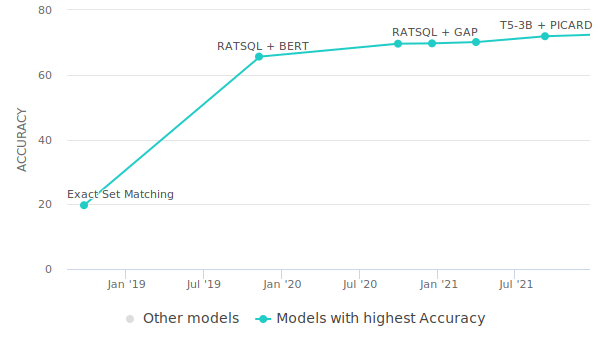
\includegraphics[page=1,width=0.7\textwidth]{pics/picard/benchmark.pdf}
%     \caption{Benchmark results for the PICARD model\cite{picard2020picard}}
% \end{figure}

After the release of Google T5, researchers have been using it to improve the accuracy of text-to-SQL models instead of BERT. New solutions have been released, such as the PICARD with T5-3B model, that significantly improved the SPIDER challenge's accuracy and are motivating researchers to use T5 in their work with innovative approaches since 2021.

\subsubsection{T5}

In Transfer Learning, we start by training our model in an unsupervised fashion on unlabeled data. Then fine-tuning it on a labeled dataset some tasks that we care about, which we call the downstream tasks. For instance, in our unsupervised free training task, we take some text, drop out some of the words, and train the model to predict the missing words. Next, we will fine-tune it on a supervised task like sentiment analysis classifying movie reviews as a given label. This way of training has become an incredible recipe for natural language processing.

T5 Model implemented by Raffel et al. (2020)\cite{raffel_exploring_2020} uses the BERT encoder-decoder architecture proposed by Vaswani et al. (2017) \cite{devlin-etal-2019-bert} and they showed in their studies that it will outperform decoder-only language models. Originally T5 was introduced with five pre-trained models — Small (60 million parameters), Base(220 million parameters), Large(770 million parameters), 3B(3 billion parameters), and 11B(11 billion parameters)\cite{raffel_exploring_2020}.

\begin{figure}[h]
    \centering
    \includegraphics[width=0.5\textwidth]{pics/picard/t5-size.png}
    \caption{T5 models with their Nr. of parameters, layer and feed-forward parameters\cite{raffel_exploring_2020}}
\end{figure}

To pre-train the T5 model, we start with clean text and drop some words to corrupt the text. Each dropped-out span will be replaced with a unique sentinel token, so if multiple words in a row get dropped out, they will be replaced with a single token. The words are dropped out independently uniformly at random so for an inviting get replaced by a single Sentinel token. Then the model is trained to output Sentinel tokens to delineate the dropped-out text corresponding to the text that was dropped out in the input and then each span of dropped-out text.

This method is pretty similar to the span BERT objective. It tried to come up with an objective that was not too different from standard practice.

\begin{figure}[h]
    \centering
    \includegraphics[width=0.6\textwidth]{pics/picard/t5-fine.png}
    \caption{Pre-training by Replace Corrupted Spans \cite{raffel_exploring_2020}}
\end{figure}

Google T5's basic idea is that it models every NLP problem and every text problem as a text-to-text task that takes the text as input and produces text as output.

So fundamentally, it is in a sequence-to-sequence framework; hence, T5 is perfectly suitable for transfer learning machine translation.
T5 can handle various tasks, and it can be fine-tuned for different NLP tasks, such as summarization, COLA (Corpus on linguistic acceptability), classification, multiple text translation, also regression problems like STSB  that predict how similar two sentences are. And in our case Text-to-SQL.

\begin{figure}[h]
    \centering
    \includegraphics[width=0.9\textwidth]{pics/picard/t5-task.png}
    \caption{Each task uses text as input in the model and generates target text. In this way, the same model, loss function, and hyper-parameters are used across various diverse tasks, including translation. \cite{raffel_exploring_2020}}
\end{figure}

Further, because the same model is used for many tasks, the model understands which tasks to perform by prepending a prefix that will also be text.
Therefore, By the end of fine-tuning, T5 will have "n" different models where "n" is the number of tasks. It starts with the same base pre-trained model, and then it is fine-tuned on task A, and then separately, on task B and task C. In our work, we are essentially adding another task to the T5 to handle SQL translation.

\subsubsection*{C4 (Colossal Clean Crawled Corpus)}

The T5 model is pre-trained on C4 Dataset\cite{raffel_exploring_2020}, so its results are quite realistic.
The C4 is an unlabeled dataset gathered and filtered from Common Crawl Dataset, a non-commercial crawler that saves snapshots of the web every month. And web content is dumped out on the order of 20 terabytes.

The cleaning process included deduplication, discarding incomplete sentences, and removing offensive or noisy content. The filtering led to more reliable results on downstream tasks, and the added size let the model size grow without over-fitting when pre-training. C4 is about 750 gigabytes of clean-ish data and is accessible in Tensorflow Datasets Library.


\subsubsection*{Beam Search}
Before understanding the PICARD, let us first understand the concept of Beam Search:

\begin{figure}[h]
    \centering
    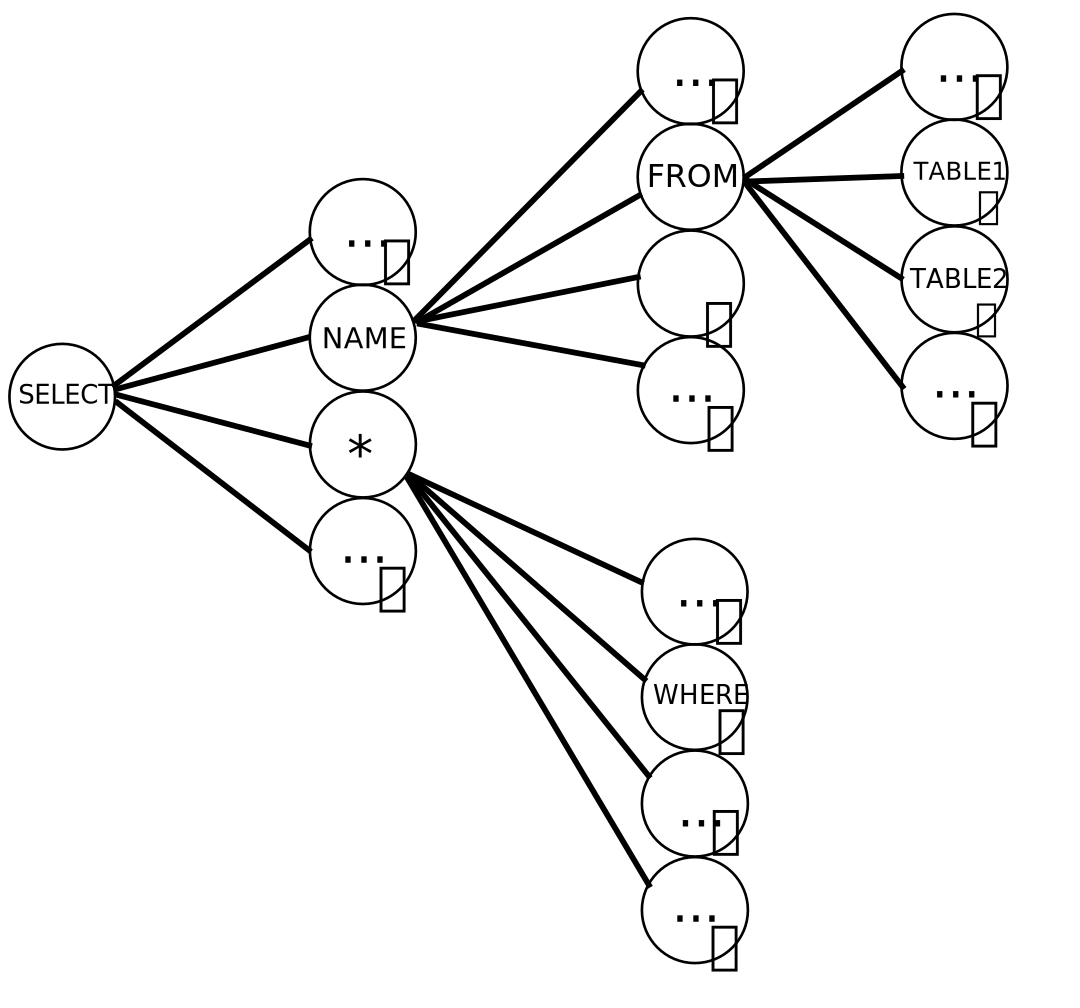
\includegraphics[width=0.6\textwidth]{pics/picard/beam.png}
    \caption{4-Beam Search}
    \label{fig:beam_search}
\end{figure}

Beam search is a widely used search algorithm in natural language processing and machine learning. It is beneficial in sequence-to-sequence (seq2seq) models, which generate output sequences based on input sequences. Beam search is used to find the most likely sequence of output words given an input sequence.
\\
The basic idea behind beam search is to maintain a set of the most likely sequences at each step of the decoding process. This set of sequences, called the "beam," is initially set to the starting point of the decoding process, and at each step, new sequences are generated by considering all the following possible words. The new sequences are then ranked based on their likelihood, and the highest-ranking sequences are added to the beam. The process is repeated until a stopping criterion is met \cite{10.1371/journal.pone.0211558}.
Beam search is handy in seq2seq models because it allows the model to generate multiple output sequences rather than just a single sequence. This is important because, in many cases, there may be multiple valid outputs for a given input sequence. By generating multiple outputs, beam search allows the model to explore the space of possible outputs and find the most likely sequences.
\\
One of the critical advantages of beam search is that it is computationally efficient. Because it only considers a small number of sequences at each step, it can quickly find the most likely sequences without exploring the entire space of possible outputs. This makes it well-suited for use in applications with limited computational resources, such as on mobile devices or in real-time systems.
Another advantage of beam search is that it can be used with other techniques, such as attention mechanisms, to improve the performance of seq2seq models. Attention mechanisms allow the model to focus on specific parts of the input sequence when generating the output, which can help to improve the quality of the generated sequences.
\\
In conclusion, Beam Search is a robust algorithm widely used in natural language processing and machine learning, particularly in the context of sequence-to-sequence (seq2seq) models. It allows the model to generate multiple output sequences rather than just a single sequence and is computationally efficient, making it well-suited for use in applications where computational resources are limited. Additionally, it can be combined with other techniques, such as attention mechanisms, to improve the performance of seq2seq models.

\subsubsection{PICARD}

% PICARD\cite{Scholak2021:PICARD} stands for "Parsing Incrementally for Constrained Auto-Regressive Decoding.". It can be used with any existing language model decoder or vocabulary based on auto-regressive language modeling.

% PICARD allows for the generation of executable code by constraining the output of the language model to be syntactically and semantically correct. It does this by integrating with standard beam search, a technique used in natural language processing to generate a sequence of words or tokens by expanding a beam of hypotheses step by step. At each decoding step, PICARD checks whether the most likely tokens are valid and if not, it discards them. PICARD is compatible with any model that generates a sequence of tokens and can be used with character, subword, and word-level language models without requiring exceptional recovery.

PICARD\cite{Scholak2021:PICARD}, short for "Parsing Incrementally for Constrained Auto-Regressive Decoding," is a method that can be used in conjunction with any language model decoder or vocabulary that utilizes auto-regressive language modeling.

PICARD is a technique that utilizes standard beam search, commonly used in natural language processing, to generate executable code by ensuring the output of the language model is both syntactically and semantically correct. It works by expanding a beam of hypotheses step by step and discarding any tokens that are not valid at each decoding step. This method can be applied to any language model that generates a sequence of tokens, including character, subword, and word-level models, without requiring unique recovery methods.

It effectively improves the performance of existing models and achieves state-of-the-art performance on tasks such as text-to-SQL translation.
Warps model prediction scores and integrates trivially with existing greedy and beam search algorithms used in auto-regressive decoding from language models.

At each generation step, Picard first restricts prediction to the top-k highest probability tokens and then assigns a score of negative infinity to those that fail Picard's numerous checks.

PICARD has four modes that control the level of comprehensiveness of its checking process: off, lexing, parsing without guards, and parsing with guards, with the latter being the most comprehensive. In lexing mode, PICARD checks if the current token is a valid keyword or identifier. In parsing guard mode, it checks if the current token is a valid keyword or identifier, a valid SQL keyword, and a valid SQL identifier.

Picard can detect spelling errors in keywords or reject table and column names that are invalid for the given SQL schema.
"Out-of-distribution compositional generalization and natural language variation" refers to the ability of a natural language processing (NLP) system to handle novel combinations of words and phrases that it has not seen before while also being able to handle variations in language usage.
Compositional generalization refers to the ability of an NLP system to understand and generate novel combinations of words and phrases by using its knowledge of the meanings and relationships of individual words and phrases. This is an essential aspect of NLP because it allows the system to understand and generate language flexibly and adaptively.

The concept of natural language variation refers to the multiple ways people can express the same ideas or concepts using natural language. This can include variations in dialect, style, or tone, which can make it difficult for NLP systems to understand and generate language accurately.

Together, out-of-distribution compositional generalization and natural language variation represent fundamental challenges in the field of NLP. They require NLP systems to handle a wide range of language input and output in order to be effective.

PICARD can be applied as an optional feature during inference but is not necessarily included in pre-training or fine-tuning, and for text-to-SQL translation, it works directly on the output of the language model. PICARD has been shown to have state-of-the-art performance on complex Spider text-to-SQL translation tasks, achieving an accuracy of 75.1\%.

Picard warps model prediction scores and integrates trivially with existing greedy and beam search algorithms. In addition to the token ids of the current hypothesis, the model's language modeling head also predicts the log-softmax scores for each vocabulary token. Additionally, Picard has access to SQL schema information, including table and column names and which column resides in which table.

Motivated by the success of Shaw et al. \cite{shaw-etal-2021-compositional}, who demonstrated that a pre-trained T5-Base or T5-3B model could effectively learn the text-to-SQL task, generalize to never-before-seen databases, and even rival the state-of-the-art methods of Choi et al.\cite{10.1162/coli_a_00403} without any modifications to the model itself, the researchers opted to use T5 as the baseline for all their experiments. The results from Shaw et al.\cite{shaw-etal-2021-compositional} suggest that T5-based models had the potential to improve the field of natural language processing significantly. Therefore, the researchers sought to take advantage of the capabilities of T5 in order to gain new insights into how natural language can be effectively utilized to solve complex tasks.
\subsection{RASAT}

RASAT \cite{https://doi.org/10.48550/arxiv.2205.06983}